\documentclass[10pt]{article}
\usepackage{graphicx}

\title{Characterization of Demographic Inclusiveness in Human Cell Studies}
\author{Jessica Snyder\textsuperscript{1}, Iva Bojic\textsuperscript{1}, Carlo Ratti\textsuperscript{1}}

\begin{document}
 \maketitle
  
   \begin{center} \textsuperscript{1}Senseable City Lab, Department of Urban Studies and Planning, Massachusetts Institute of Technology, \\* \\* 77 Massachusetts Ave. Cambridge, MA 02141, USA  \end{center} \\* \\* 
  
\hline
\section*{Abstract}
The possibility of demographic bias in cell culture studies specifically the gender, age and ethnicity of human donors supplying to the cells used for research can have significant consequences for the validity of findings during early stage pharmaceutical studies. The research process for preclinical studies typically progresses from cell models, to animal models, and finally human models. During the cell model stage, donors provide a sample of cells to be grown in a lab environment. Federal regulations require broad spectrum representation of gender, age and ethnicity during the final phase of clinical testing, the human model stage. Iva and I have been discussing how demographic factors during the earlier cell model stage may be significant as well. What criteria do biologists use when selecting cell sources for early studies? Is there a quantifiable bias in extant literature for cell model studies? 

\\* \\* \textit{Keywords:} Cell study \\* \\*  \hline


\section{Introduction: Objectives and significance}

The human genome's major structures recur across the global population regardless of geographical ancestry, self-identified race or sociocultural considerations \cite{xie2001molecular, cooper2003race}. Still, comparatively minor genetic variants generate predictable  alterations in the therapeutic impact of some pharmaceutical treatments. Clustering patients by genotype informs the course of drug therapies during treatment of cancer and organ transplant \cite{krynetski2000genetic, higashi2002association}. The most significant pharmacokinetic variability comes from alterations to drug-metabolizing enzymes and metabolic pathways caused by genetic polymorphism \cite{bjornsson2003conduct, naito1998ethnic}. 

The US Food and Drug Administration (FDA) recognized genetic factors sensitize pharmaceutical efficacy and responded by implementing the Demographic Rule in 1998.  The rule standardizes race and ethnicity representative during clinical trails based on the target therapeutic population as identified by the drug's sponsor. The FDA utilizes ethnicity as a population-level sorting method for inclusion, extrinsic (concomitant medications, nutrition, physical activity) and intrinsic  (genetics, enzyme expression, renal and hepatic function) health metrics \cite{yasuda2008role}. Racial and ethnicity diversity serves as an unsubstantiated proxy for broad spectrum representation of genetic variants during clinical trials \cite{haga2003fda}. Generalizations of drug-sensitivity along ethnic group assume the attributable extrinsic or intrinsic factors persist across the group \cite{roy2005cyp3a5}. The variation within ethnic groups may well be greater within a group than the between them. 

Demographically representative genomic sampling promotes equal access to a research project's anticipated value \cite{jackson1999african}.  Patient involvement during early research of therapeutic development prioritizes patient-centered outcomes \cite{hoos2015partnering}. Extrinsic factors such as body weight most significantly modulated individual variability of anti-body-drug conjugate pharmacokinetics to treat metastic breast cancer \cite{gupta2012clinical}.

Of 185 drug products audited by the FDA, 10\% disclosed differences related to race in the efficacy or toxicity of the pharmaceutical on the label \cite{evelyn2001participation}. The predominant drug class to disclose racial sensitivity being cardio-renal, followed by neuropharmacology and metabolic/endocrine \cite{evelyn2001participation}. 


Intrinsic and extrinsic factors modulate the effectiveness and dose of a particular drug. Extrinsic factors (concomitant medications, nutrition, physical activity) and several intrinsic factors (age, weight) modulate physiology across length-scales much larger than an individual cell or tissue. Several intrinsic factors (genetics, enzyme expression, renal and hepatic function) drive physiology in length-scales of a single cell or several cell assembly and are also known to generate mechanistic changes in drug response. Genetic variability in drug-metabolizing enzymes is one of the most significant sources of variability during drug exposure \cite{bjornsson2003conduct}.  An example of a ethnic-sensitivity to drug efficacy due to differentially expressed metabolic pathways is the immunosuppressive drug tacrolimus and pathways CYPA5 and CYPA - differentially expressed in African-American and white populations  \cite{roy2005cyp3a5}.

US Food and Drug Administration (FDA) implemented the Demographic Rule in 1998 to standardize the inclusion of race and ethnicity representation representative of the target therapeutic population during clinical trails.  

The Human Genome Project's strategy includes human sequence variation to foster inclusion. Whole genome perspectives on population-level genetic variation between individuals are based on multiple historical sources \cite{foster2004beyond}. 

Variation inclusive genome databasing 

The European Commission (EC) and National Institute of Health led the formation of an international traumatic brain injury recognized compounding extrinsic factors demanded broad spectrum demographic inclusion \cite{tosetti2013toward}.

Designing transformative clinical trials for the cancer genome era \cite{sleijfer2013designing}.

Social media facilitates social support for breast cancer patients to increase perceived knowledge and decrease anxiety  \cite{attai2015twitter}.

The Food and Drug Administration (FDA) pharmaceutical approval process cannot fully anticipate rare adverse events. Crowdsourcing introduces rating systems and fails to fully mitigate public health risk of drugs \cite{darrow2014crowdsourcing}.

Body weight most significantly modulated individual variability of anti-body-drug conjugate pharmacokinetics to treat metastic breast cancer \cite{gupta2012clinical}.

Address perceptions racial and ethic groups are under-represented during clinical trials of new drugs. Race-related labeling for new molecular entities  \cite{evelyn2001participation}

Retrospective FDA review of clinical trial protocols 

Enrollment data Racial representation during new molecular entity (NME) testing by the year of the clinical trial and therapeutic category 

A retrospective of the US Food and Drug Administration (FDA)'s review of clinical trail protocols identified 10\% of the 185 products approved from 1995-1999 disclosed racial differences in the performance of the product on the label \cite{evelyn2001participation}.  Cardio-renal, neuropharmacology and metabolic/endocrine drug classes 




An FDA audit clinical trail protocols those conducting the clinical trial disclosed the race of participants for 53\% of the nearly 500k individuals enrolled in clinical trials from 1995 - 1999  \cite{evelyn2001participation}.  Of the 260k participants whose race was specified, white was most common (88\%), African American was comparable to US population percentage (8\%), and the report classified hispances as underrepresented with 1\% of participants.  Within drug classes the distribution of demographic shifted from more inclusive (specific pathogen and anti-infective drug) to less inclusive (neuropharmacological, pulmonary and oncologic drug trials).  


\\* \\*  \textbf{The research objective of this proposal is to characterize the demographic inclusiveness of human cell sources for cell studies during the preliminary stages of drug development.}  To accomplish the overall goal two research tasks are defined. 
\textbf{First}, query the Directory of Open Access Journals (DOAJ) to generate a set of demographic descriptors of donors whose cells were utilized in peer reviewed studies. \textbf{Second}, utilize the data set to characterize the representation of gender and ethnicity by research topic over the span of available years. 

\\* \\* The proposed work \textbf{aligns with current effort} to vet the efficacy and toxicity of drug candidates early in the discovery process. Proportioned demographic diversity early in the discovery process may mediate the optimal drug candidate or result in multiple tailor-made candidates. The \textbf{intellectual merit} of the proposed research lies in expanding the decision criteria for cell sources during the discovery process for an abridged implementation of personalized medicine. The \textbf{broader impact} of the proposed research is in its potential to enhance knowledge of inefficiencies within the drug discovery process. 

\section{Background}

\section{Preliminary studies}

\section{Research plan}
\subsection{Task #1: Generate data set}
Query the Directory of Open Access Journals (DOAJ) to generate a set of demographic descriptors of donors whose cells were utilized in peer reviewed studies. Table~\ref{table:DataFields} presents examples of data fields relevant to accomplishing the aims of this study. 

\subsubsection{Rationale}
\subsubsection{Experimental design}
\subsubsection{Expected outcomes and alternative approaches}


\begin{table}[!t]
\caption{Data fields required to assess demographic representation for human cell studies. Standard ethnicity categories defined by the US FDA Office of Management and Budget.}
\centering
\begin{tabular}{c c l l }
\hline 
  & No. & Term & Sub-categories  \\
\hline 
Query & 1 & Peer reviewed publication  &  \\
& 2 & In vitro cell study  &  \\
& & Human primary cells &  \\
\hline
Collect&1 & Publication metadata &  \\
&2 & Donor Gender & Female \\
& & & Male \\
&3 & Donor Ethnicity & Hispanic or Latino   \\
& & & Not Hispanic or Latino  \\
&4 & Donor Race & African American\\
&&& American Indian or Alaska Native  \\
&&& Asian \\
&&& Black \\
&&& Native Hawaiian or other Pacific Islander \\ 
&&& White   \\
&5 & Donor Age &  (years) \\
\hline
\end{tabular}
\label{table:DataFields}
\end{table}

\subsection{Task #2: Visualization}
Utilize the data set to characterize the representation of gender and ethnicity by research topic over the span of available years. 

\begin{figure}[!t]
\centering
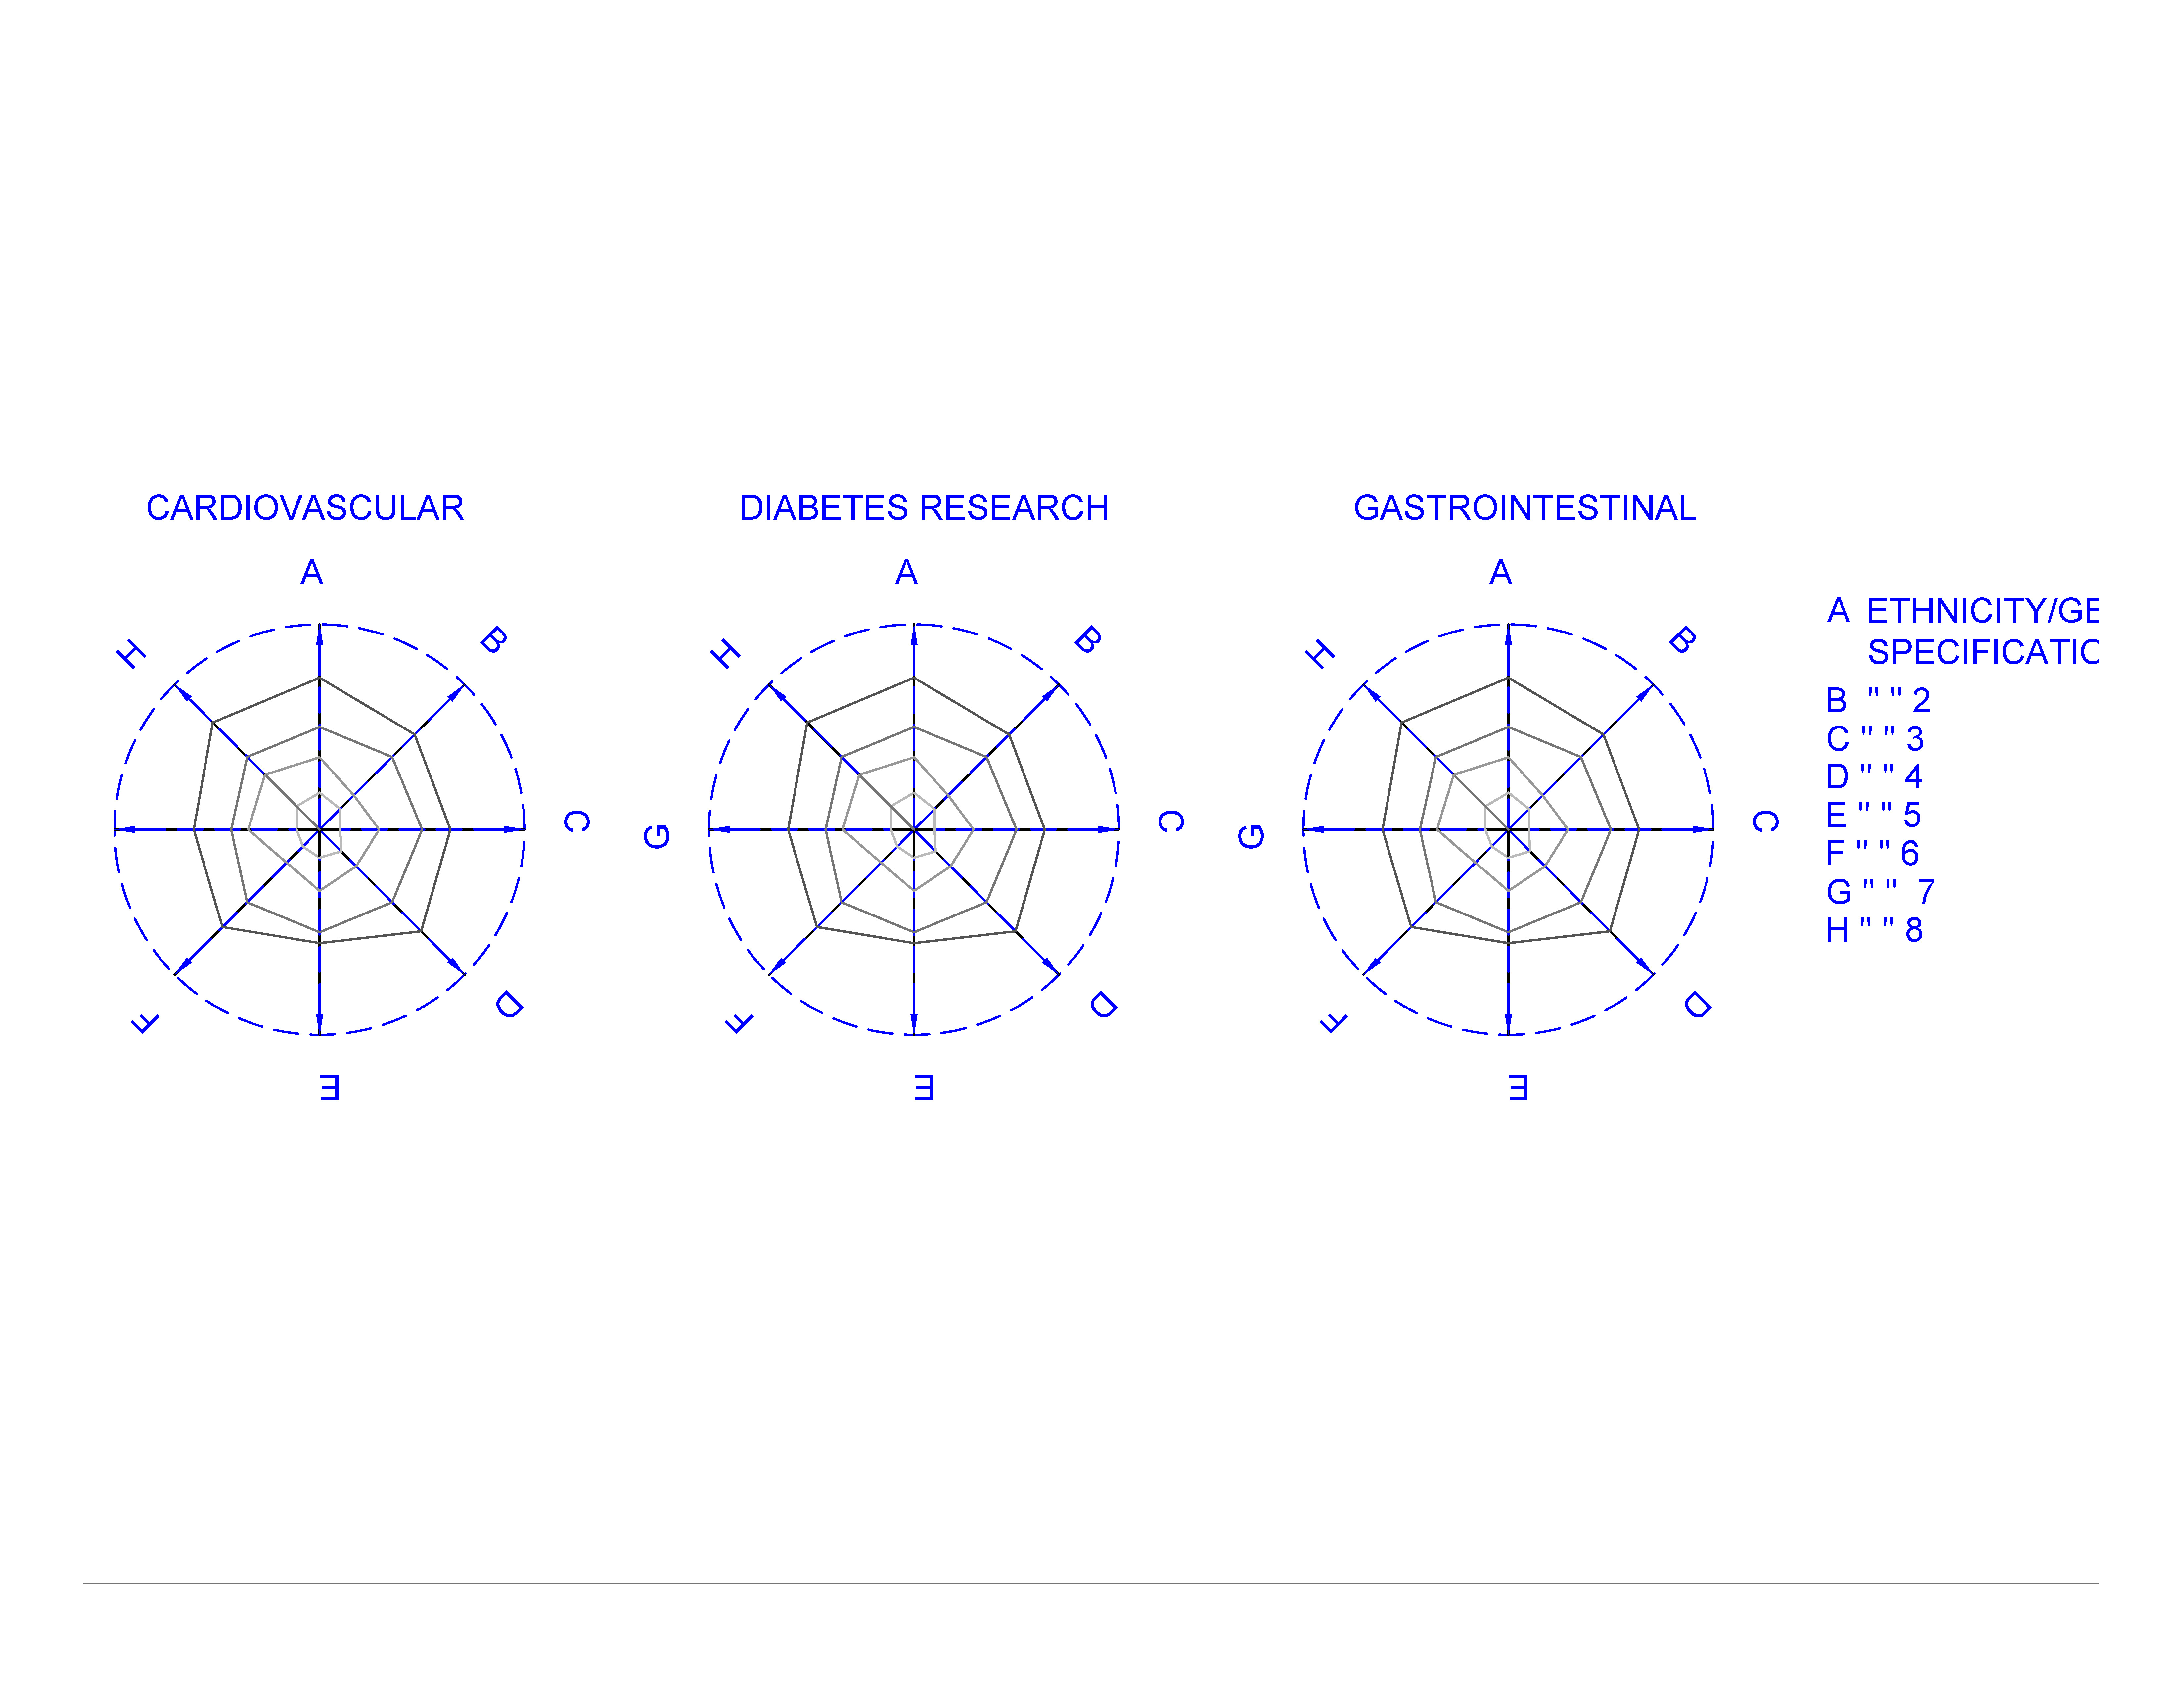
\includegraphics[trim={0 200 0 150},clip, width=1\textwidth]{EBDemo}
\caption{Cumulative numbers of studies for each ethnic and gender specification.}
\label{figure:GISmap}
\end{figure}

\subsubsection{Rationale}
\subsubsection{Experimental design}
\subsubsection{Expected outcomes and alternative approaches}

\section{Conclusion}

\section*{Aknowledgements}


\bibliographystyle{unsrt}
\bibliography{refs}


\enddocument